\documentclass[10pt,a4paper]{report}
\usepackage[utf8]{inputenc}
\usepackage{amsmath}
\usepackage{amsfonts}
\usepackage{amssymb}
\usepackage{graphicx}
\newcommand{\omegav}{{\bf \omega}}
\newcommand{\xv}{{\bf x}}
\newcommand{\et}{{\bf e}_\theta}
\newcommand{\alphav}{{\bf \alpha}}
\begin{document}
\begin{huge}
Simulation of Toroidal Vortex Ring(From Ghoniem's paper\cite{ghoniem})
\end{huge}
\section{Geometry and Initial Vorticity Distribution}

Here we look at a toroidal vortex ring with an initial vorticity distribution modeled by a third order Gaussian function:
\begin{equation}
\omegav (\xv) = \frac{1}{a\sigma^2} exp\left(-r_\xv^3/\sigma^3\right) \et
\end{equation} 
\begin{figure}
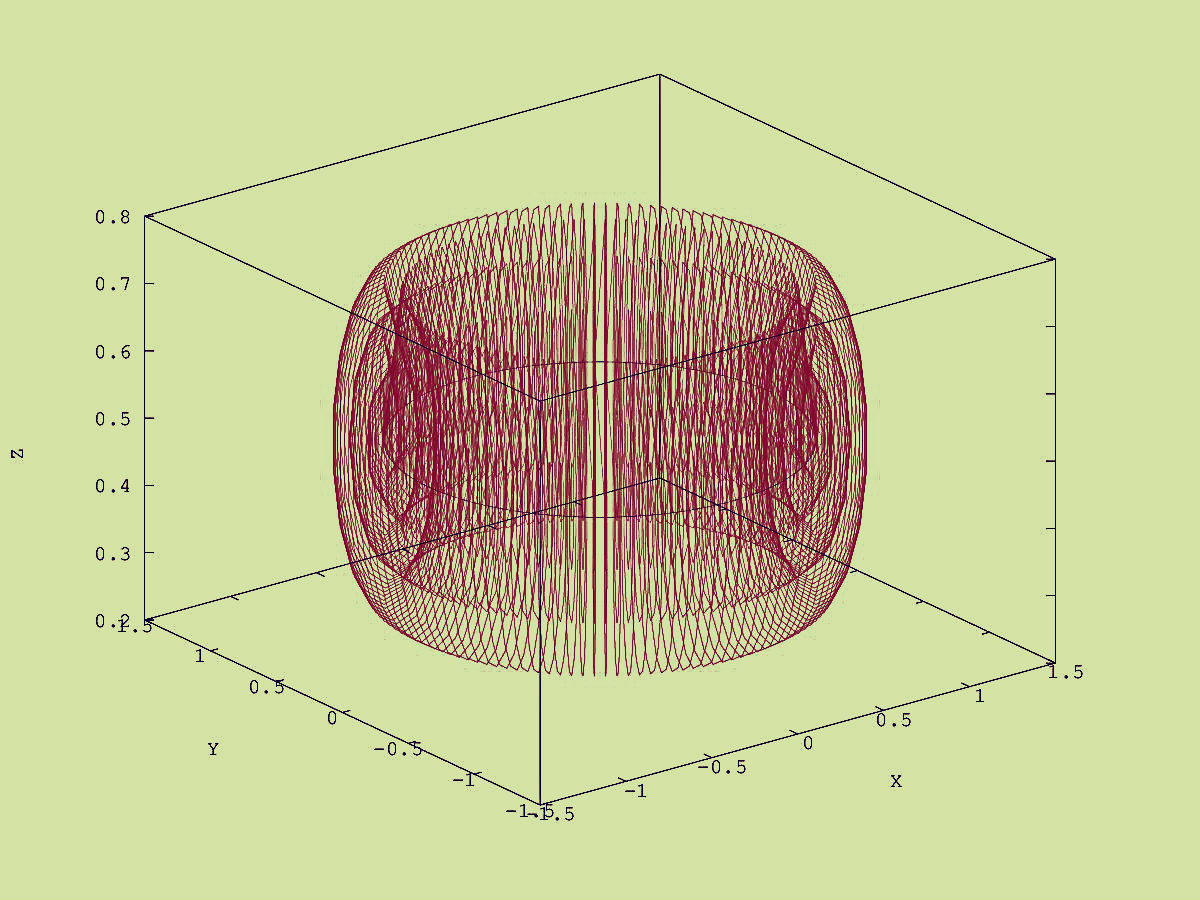
\includegraphics[scale=0.3]{geometry.jpg}
\caption{Vortex Torus with ring axis in blue}
\end{figure}
The vorticity is along the direction $\et$ which is tangential to the ring axis(shown in the figure). The ring axis is the circle, $x^2 + y^2 = R^2$ on the plane $z=z_i$.
The magnitude of the total vorticity is independent of $\theta$ where $(\rho,\theta, z)$ are represent coordinates in the cylindrical coordinate system.
\paragraph{}
The cross section of the ring, which is circular, has a radius, $\sigma = 0.275 R$. In the figure, $R = 1$ and $z_i = 0.5$.
\paragraph{}
In a particular cross section,
\begin{itemize}
\item
$r$ is the radial distance measured from the centre of the core of the ring or the centre of a cross section. For all $\xv$ within the ring, $0 \leq r_\xv \leq \sigma $ . 
\item
$\phi$ is the angle measured, at every cross section, from the line passing through the centre of the cross section and parallel to the z axis.  
\end{itemize}
\begin{figure}
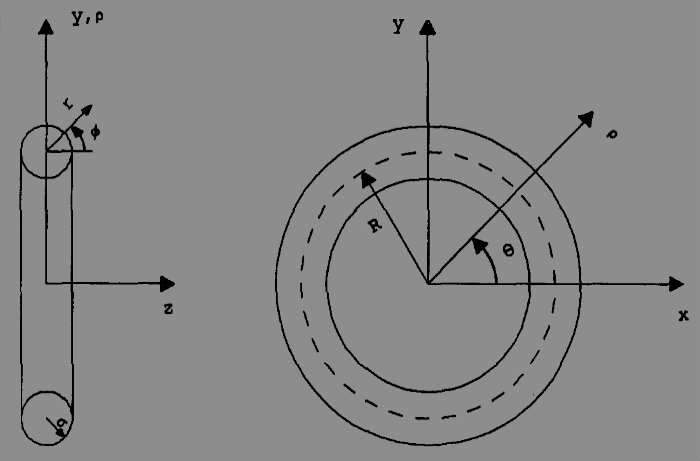
\includegraphics[scale=0.3]{axis.jpg}
\caption{From \cite{Ghoniem}}
\end{figure}

\section{Discretization of the Ring}

The toroidal ring is divided into many small vortex tubes. Here, we make an equi-spaced mesh found in the third position on the third row of Fig.11 b of the paper\cite{ghoniem}. The ring is discretized at $N_c$ cross sections and each cross-section is discretized at $N\_per\_ \theta$ locations in total.

Of these $N\_per\_ \theta$ locations, $N_\theta $ points are at each radial location and there are $N_r $ radial locations per cross section. 

In the code, $N_r = 3$ and $N_\theta $ is a multiple of 6. Hence, there are $ N\_per\_\theta = 1 + 6 + 12 + 18 = 37$ elements (including one at the centre) in total per cross section. 

Therefore, the ring is divided into $N = N_c \times N\_per\_\theta $ vortex tubes in total. In the code, $N_c = 120$. Hence, we have $4440$ vortex elements which are part of $N\_per\_\theta $ different vortex tubes.

\begin{figure}
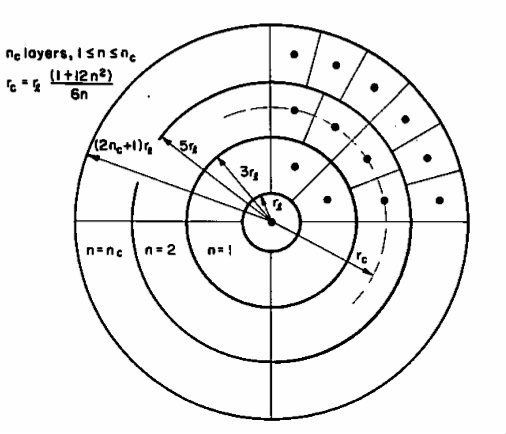
\includegraphics[scale=0.4]{discrete.jpg}
\caption{From \cite{wincklemans} }
\end{figure}

\section{Evaluating Strength Vectors}
In a regularized particle vortex method, the total vorticity field at a given $\xv$ at time t is written as:
\begin{equation}
\oemgav(\xv, t) = \sum_{i=1}^N \alphav
\end{equation}








\begin{thebibliography}{3}
\bibitem{ghoniem} 
\emph{Omar M. Knio and Ahmed F. Ghoniem},Numerical Study of a Three Dimensional Vortex Method,
Journal of Computational Physics,1990

\bibitem{wincklemans}
\emph{G.S. Wincklemans and A. Leonard}
,Contributions to Vortex Particle Methods for the Computation of Three-Dimensional Incompressible Flows,
Journal of Computational Physics, 1993.

\end{thebibliography}

 



 
\end{document}